\begin{enumerate}
 \item On veut prouver ici que la fonction $n$ est décroissante. Considérons deux réels $r_1$ et $r_2$ avec $0<r_1<r_2$, et une $r_2$-configuration de $n_2$ sphères avec $n_2=n(r_2)$. Formons, dans chaque sphère de cette configuration une sphère de même centre mais de rayon $r_1$. Ces shères sont disjointes mais elles ne sont plus tangentes à la sphère unité. Translatons chacune d'un vecteur de longueur $r_2-r_1$ dans la direction du centre de la sphère unité. Elles sont alors tangentes à la sphère unité mais malgré ce que laisse croire la figure \ref{fig:Csphertan_1}, le fait qu'elles soient deux à deux disjointes  doit être justifé.

\begin{figure}[h!t]
 \centering
 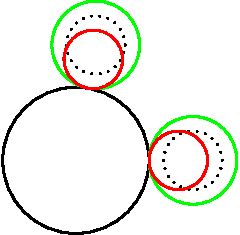
\includegraphics{./Csphertan_1.pdf}
 \caption{La fonction $n$ est décroissante.}
 \label{fig:Csphertan_1}
\end{figure}
Notons $U_2$ et $V_2$ les centres de deux quelconques des sphères de la $r_2$-configuration et $u$, $v$ les vecteurs unitaires associés. Notons $U_1$ et $V_1$ les centres des sphères obtenues par les opérations indiquées.
\begin{displaymath}
U_2 = O + (1+r_2)u,\hspace{0.5cm} V_2 = O + (1+r_2)v,\hspace{0.5cm} U_1=O+(1+r_1)u,\hspace{0.5cm} V_1=O+(1+r_1)v 
\end{displaymath}
On en déduit $U_1V_1=(1+r_1)\Vert u-v\Vert$ et $U_2V_2=(1+r_2)\Vert u-v\Vert$ d'où
\begin{displaymath}
 U_1V_1 = \frac{1+r_1}{1+r_2}\,U_2V_2 \geq \frac{1+r_1}{1+r_2}r_2 > r_1 
\text{ car }
\frac{1+r_1}{1+r_2}r_2 - r_1 = \frac{r_2-r_1}{1+r_2}>0
\end{displaymath}
Les sphères ainsi fabriquées forment donc une $r_1$-configuration ce qui assure que $n(r_1)\geq n(r_2)$.  
 \item Pour montrer que $n(r)\geq2$ pour tous les $r$, il suffit de trouver une $r$-configuration de deux sphères. Considérons un vecteur unitaire $u$. Les sphères de rayon $r$ et de centre $O+(1+r)u$ et $O-(1+r)u$ sont dans des demi-espaces disjoints, elles forment donc une $r$-configuration.
 \item Introduisons les vecteurs unitaires et $\theta_{ij}$ l'écart angulaire entre ces vecteurs.
\begin{displaymath}
 \left. 
\begin{aligned}
\overrightarrow{OA_i} = (1+r)u_i \\
\overrightarrow{OA_j} = (1+r)u_j 
\end{aligned}\right\rbrace 
\Rightarrow
\Vert \overrightarrow{A_iA_j}\Vert^2 = (1+r)^2\Vert u_i - u_j\Vert^2
= (1+r)^22(1-\cos \theta_{ij})
\end{displaymath}
Comme les sphères ne se coupent pas:
\begin{displaymath}
 (1+r)^22(1-\cos \theta_{ij})\geq (2r)^2 \Rightarrow
1-\cos \theta_{ij} \geq \frac{2r^2}{(1+r)^2} \Rightarrow
\cos \theta_{ij} \leq 1-\frac{2r^2}{(1+r)^2}
\end{displaymath}

 \item
\begin{enumerate}
 \item Considérons une $r$-configuration de $3$ sphères. Notons encore $\theta_{ij}$ les écarts angulaires entre les vecteurs dirigés vers les centres et développons le produit scalaire indiqué. On obtient
\begin{displaymath}
 \Vert \sum _{i=1}^{3}\overrightarrow{OA_i}\Vert^2
= (1+r)^2(3+2\cos \theta_{12}+2\cos \theta_{13}+2\cos \theta_{23})
\end{displaymath}
Comme il s'agit d'une $r$-configuration, on peut majorer les $\cos$, on en tire
\begin{displaymath}
 0 \leq 3(1+r)^2\left (1+2(1-2\frac{r^2}{(1+r)^2}) \right)
\Rightarrow
-r^2 + 6r +3 \geq 0
\end{displaymath}
Le polynôme du second degré admet deux racines réelles $3- 2\sqrt{3}<0<3+ 2\sqrt{3}$. Comme $r>0$, cela entraine $r\geq 3+ 2\sqrt{3}$.\newline
On vient de montrer que l'existence d'une $r$-configuration de 3 sphères entraine $r\geq 3+ 2\sqrt{3}$. Par contrapposition, cela signifie aussi que $r< 3+ 2\sqrt{3}$ entraine qu'il n'existe pas de $r$-configuration de $3$ sphères c'est à dire que $n(r)<3$. Comme il existe toujours des configurations de $2$ sphères, on doit avoir $n(r)=2$.
 \item Le raisonnement est analogue. On commence par considérer une configuration de $4$ sphères et on développe le carré indiqué. On en tire (en majorant les $\cos$)
\begin{displaymath}
 0 \leq (1+r)^2\left (4+12(1-2\frac{r^2}{(1+r)^2}) \right)
\Rightarrow
-r^2 + 4r +2 \geq 0
\end{displaymath}
Le polynôme du second degré admet deux racines réelles $2- \sqrt{6}<0<2+ \sqrt{6}$. Comme $r>0$, cela entraine $r\geq 2+ \sqrt{6}$. On termine comme dans la question précédente.
\end{enumerate}

 \item
\begin{enumerate}
 \item Par des considérations de géométrie élémentaire ou par des calculs avec des nombres complexes (calcul du module de $1-j$ par exemple), on trouve que la distance entre deux sommets d'un triangle équilatéral inscrit dans un cercle de rayon $R$ est $R\sqrt{3}$.\newline
Dans un plan de l'espace, inscrivons un triangle équilatéral dans un cercle de rayon $1$. La distance entre les sommets est $\sqrt{3}$. Formons des sphères de rayon $\frac{\sqrt{3}}{2}$ centrées en ces $3$ sommets. Elles ne se coupent pas et sont tangentes à la sphère centrée à l'origine et de rayon $1-\frac{\sqrt{3}}{2}$.  Par une homothétie de centre $O$ et de rapport l'inverse de $1-\frac{\sqrt{3}}{2}$, on construit une $r$-configuration de $3$ sphères avec
\begin{displaymath}
 r = \frac{\frac{\sqrt{3}}{2}}{1-\frac{\sqrt{3}}{2}}
= \frac{\sqrt{3}}{2-\sqrt{3}}= \sqrt{3}(2+\sqrt{3}) = 3+2\sqrt{3}
\end{displaymath}
Ainsi, pour $r=3+2\sqrt{3}$, il existe une $r$-configuration de $3$ sphères ce qui entraine que $n(3+2\sqrt{3})\geq3$ et, par décroissance de $n$,
\begin{displaymath}
 r\leq 3+2\sqrt{3} \Rightarrow n(r) \geq 3
\end{displaymath}

 \item La méthode est la même pour les questions 5 a. et b. On considère $m$ points tous à la même distance $R$ de l'origine. Dans la question a., ils sont équidistants entre eux mais dans les autres cas, on connait seulement la plus petite distance $d$ entre deux de ces points. Les $m$ sphères de rayon $r=\frac{d}{2}$ et centrées en ces points  sont donc tangentes ou disjointes. De plus, elles sont tangentes à la sphère centrée à l'origine et de rayon $R-r$. En utilisant l'homothetie de centre l'origine et de rapport $\frac{1}{R-r}$, on obtient une $\frac{r}{R-r}$\,-configuration de $m$ sphères ce qui prouve que $n(\frac{r}{R-r})\geq m$.\newline
Dans cette question, $m=4$, $R=\sqrt{3}$, $d=2\sqrt{2}$:
\begin{displaymath}
 \frac{r}{R-r}=\frac{\sqrt{2}}{\sqrt{3}-\sqrt{2}}=\sqrt{2}(\sqrt{3}+\sqrt{2})
\text{ d'où }
r\leq 2+\sqrt{6} \Rightarrow n(r) \geq 4
\end{displaymath}
par décroissance de $n$.

 \item On utilise dans chaque cas la méthode et les notations précisées en a.\newline
\emph{Cas des sommets du cube} : $m=8$ avec les points de coordonnées
\begin{multline*}
 (1,1,1), (1,1,-1), (1,-1,1), (1,-1,-1), (-1,1,1), (-1,1,-1),\\ (-1,-1,1), (-1,-1,-1)
\end{multline*}
Donc $R=\sqrt{3}$, $d=2$ . La plus petite distance est réalisée pour deux points avec deux coordonnées égales c'est à dire reliés par une arête.
\begin{displaymath}
 \frac{r}{R-r}=\frac{1}{\sqrt{3}-1}= \frac{1+\sqrt{3}}{2}
\text{ d'où }
r\leq \frac{1+\sqrt{3}}{2} \Rightarrow n(r) \geq 8
\end{displaymath}
\emph{Cas des milieux des arêtes} : $m=12$. Une arête est une paire de points avec deux coordonnées égales. Pour l'égalité, il y a 3 couples de coordonnées possibles $(1,2)$, $(1,3)$, $(2,3)$. Pour chaque couple : 4 valeurs possibles (avec des $1$ et des $-1$) pour les coordonnées. On obtient donc bien $12$ arêtes, pour chaque milieu, la coordonnée qui n'est pas fixée est forcément nulle. Les $12$ milieux sont donc les points de coordonnées
\begin{multline*}
 (1,1,0), (1,-1,0), (-1,1,0), (-1,-1,0),\\ (1,0,1), (1,0,-1), (-1,0,1), (-1,0,-1)\\
(0,1,1), (0,-1,1), (0,1,-1), (0,-1,-1)
\end{multline*}
Donc $R=\sqrt{2}$, $d=\sqrt{2}$ : 
\begin{displaymath}
 \frac{r}{R-r}=\frac{\frac{\sqrt{2}}{2}}{\frac{\sqrt{2}}{2}}= 1
\text{ d'où }
r\leq 1 \Rightarrow n(r) \geq 12
\end{displaymath}
\emph{Cas des milieux des faces} : $m=6$. Une face est caractérisée par la valeur d'une seule coordonnée qui peut être $1$ ou $-1$ ce qui explique bien pourquoi il y en a $6$. Les deux autres coordonnées d'un milieu sont nulles les coordonnées des $6$ milieux des faces  sont donc
\begin{displaymath}
 (1,0,0), (-1,0,0), (0,1,0), (0,-1,0), (0,0,1), (0,0,-1)
\end{displaymath}
 Donc $R=1$, $d=\sqrt{2}$ :
\end{enumerate}
\begin{displaymath}
 \frac{r}{R-r}=\frac{\frac{\sqrt{2}}{2}}{1-\frac{\sqrt{2}}{2}}= 1+\sqrt{2}
\text{ d'où }
r\leq 1+\sqrt{2} \Rightarrow n(r) \geq 6
\end{displaymath}

\begin{figure}[h!t]
 \centering
 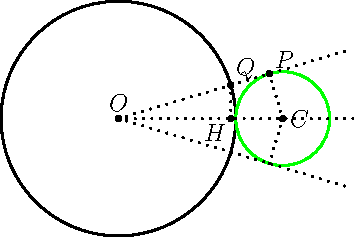
\includegraphics{./Csphertan_2.pdf}
 \caption{Aire découpée sur la sphère unité.}
 \label{fig:Csphertan_2}
\end{figure}
 
 \item
\begin{enumerate}
 \item Par symétrie du problème, on peut supposer que le centre de la sphère $S_i$ que l'énoncé nous demande de considérer est sur l'axe des abscisses. On est donc ramené à une région de la sphère unité du type considéré par l'énoncé avec $s=OH$ égal à l'abscisse du point $H$ de la figure \ref{fig:Csphertan_2}. Notons $\alpha$ l'écart angulaire entre $\overrightarrow{OC}$ et $\overrightarrow{OP}$. Comme $OQ=1$, on a 
\begin{displaymath}
 s = OH =\cos \alpha = \frac{OP}{OC}=\frac{\sqrt{(1+r)^2-r^2}}{1+r}=\frac{\sqrt{1+2r}}{1+r}
\end{displaymath}
Par la formule admise, on déduit que l'aire cherchée est
\begin{displaymath}
 2\pi\left(1- \frac{\sqrt{1+2r}}{1+r}\right) 
\end{displaymath}

 \item La somme des aires des régions formées sur la sphère unité par les sphères d'une $r$-configuration est inférieure à l'aire totale qui est égale à $4\pi$. On en déduit
\begin{multline*}
 n(r)2\pi\left(1- \frac{\sqrt{1+2r}}{1+r}\right) \leq 4\pi\\
\Rightarrow n(r) \leq \frac{2(1+r)}{\left(1+r-\sqrt{1+2r} \right) }
= \frac{2(1+r)\left(1+r+\sqrt{1+2r} \right)}{r^2}
\end{multline*}
\end{enumerate}

 \item Considérons le volume de la boule de rayon $1+2r$ qui contient toutes les boules d'une $r$-configuration. Il est plus grand que le volume de la boule unité et de toutes les boules de la configuration. On en tire
\begin{displaymath}
 \frac{4\pi}{3}1^3+ n(r)\frac{4\pi}{3}r^3\leq \frac{4\pi}{3}(1+2r)^3
\Rightarrow
n(r) \leq \frac{(1+2r)^3 -1}{r^3}=v(r)
\end{displaymath}

 \item En développant au premier ordre la racine carrée, on obtient
\begin{displaymath}
 a(r)=\frac{4}{r^2} + \frac{8}{r} + o(\frac{1}{r})
\end{displaymath}
On obtient directement, par la formule du binome,
\begin{displaymath}
 v(r)=\frac{6}{r^2} + \frac{12}{r} + 8
\end{displaymath}
L'inégalité obtenue à partir des aires est donc plus précise que celle obtenue à partir des volumes.
\end{enumerate}
